\chapter{Derivation of singles and accidental rate formulas}
\label{ap:singlesformula}

The formulas used for computing the rate of uncorrelated events
and the rate of accidental coincidences
are based on the statistical interpretation
of the coincidence grouping algorithm.
As mentioned in \cref{sec:coincidence}
and illustrated by \cref{fig:timeline_examples},
coincidence groups are formed by repeating the following steps:

\begin{enumerate}
    \item Find the next AD event.
        This AD event will be the ``prompt'' event of the coincidence group.
    \item Find all subsequent AD events within the desired coincidence time \tc.
        If a muon event is encountered within \tc,
        veto the entire coincidence group starting with the prompt event.
        (This additional vetoed time is accounted for in the muon veto efficiency.)
    \item Group these events together with the prompt event
        to form the coincidence group.
    \item Skip to the next AD event that is not part of the coincidence group.
\end{enumerate}

A reasonable and leading question to ask is,
Given the rate and correlations of AD events and muons,
what is the expected rate of \fold{1} or \fold{2}
(or, generally, \fold{n}) coincidences when using
this particular coincidence grouping procedure?

The model used for Daya Bay data is that muons
and the ``single'' or ``uncorrelated''
events that cause accidental backgrounds and
multiplicity vetos are truly uncorrelated and described by
Poisson statistics with rates of $R_\mu$ and $R_s$, respectively.
True correlated processes such as IBDs are neglected in this model
because their rate is $\sim 4$ orders of magnitude lower than $R_s$.

\section{Detailed derivation}

The derivation of the rate formulas can be broken down into three
conceptual parts which are actually factors that, when multiplied together,
give the desired rate:

\begin{enumerate}
    \item $R_s$: How many opportunities are there for a coincidence window to start?
    \item $P_{\text{start}}$: What is the probability that a given event will start a
        coincidence window (as opposed to falling within
        an existing coincidence window)?
    \item $P_{\text{mult}}$: Once started, what is the probability
        that the coincidence window has the desired multiplicity?
\end{enumerate}

Factors 1 and 3 are straightforward.
There are as many opportunities for coincidence windows to start
as there are uncorrelated events, so factor 1 is simply
the underlying uncorrelated event rate $R_s$.
(Again, neglecting IBDs and other backgrounds.)
Factor 3 is the probability that $n-1$ additional events occur
within the specified time interval of size \tc{}
(for a desired multiplicity of $n$), when those events occur with a rate $R_s$.
This is just the Poisson probability with mean $R_s\tc$:

\begin{equation}
    \text{Poisson}(n\vert R_s\tc) = \frac{\left(R_s\tc\right)^n}{n!}e^{-R_s\tc}.
\end{equation}
Hence, whatever is derived for Factor 2 below should be multiplied by
$R_s\text{Poisson}(n\vert R_s\tc)$ to obtain the formula for
an \fold{n} coincidence.

Factor 2, unfortunately, is more involved.
The probability that a given random AD event
is properly situated to start a new coincidence window depends on
the likelihood of other events to be far enough away in the past.
An equivalent formulation is to pick a time uniformly at random
(from among the times that lie outside muon veto windows)
and determine the probability that, if a new AD event were created
at that time, the event would \textit{not} lie within another
coincidence window.
This probability can be calculated by considering
a set of mutually exclusive situations
and summing the individual probability for each situation.
Three situations contribute the majority of the probability
and are illustrated in \cref{fig:ap_scenarios};
the next-most-likely situation is briefly examined in \cref{ap:singlesprecision}
to demonstrate its negligible likelihood.
The three situations are:

\renewcommand{\labelenumi}{(\alph{enumi})}
\begin{enumerate}
    \item There are no muons and no other AD events
        within \tc{} before the chosen event.
        This probability is computed as two Poisson probabilities of
        no events with rate $R_s$ in time \tc,
        and no events with rate $R_\mu$ in time \tc:

        \begin{align*}
            P_a &= \text{Poisson}(0\vert R_s\tc)\cdot\text{Poisson}(0\vert R_\mu\tc) \\
                &= e^{-\left(R_s + R_\mu\right)\tc}
        \end{align*}

    \item There is another AD event, E1, within \tc{}
        before the chosen event, E0,
        but it lies within an earlier coincidence window.
        This is significantly more complicated to calculate.
        Let $t_1$ refer to the time difference between E1 and E0.
        The time between uncorrelated events follows an exponential distribution,
        so the probability of E1 occurring between $t_1$ and $t_1+dt_1$ is
        $dt_1\,R_se^{-R_st_1}$.
        Examining the possibilities for this earlier coincidence window,
        which contains E1 but not E0,
        it is clear that the end of the window must be before E0,
        but not earlier than $t_1$ before E0, so that it still contains E1.
        Thus the time difference between the end of the window and E0
        must have a value between 0 and $t_1$.
        Since the coincidence window is a fixed duration \tc{},
        the event E2 which started the earlier window must occur
        between \tc{} and $\tc + t_1$ before E0.
        If more than one event occurs within that time interval,
        the requirements for the coincidence window would still be satisfied.
        The probability of at least one event (E2, E3, \ldots) occurring
        between \tc{} and $\tc + t_1$ before E0,
        and thus creating the desired coincidence window, is

        \begin{equation*}
            1-\text{Poisson}(0\vert R_s t_1) = 1-e^{-R_st_1}.
        \end{equation*}

        Finally, there must be no muon veto window ending within this time range
        between E2 and E0, which has duration $\tc + t_1$,
        leading to the Poisson probability $e^{-R_\mu(\tc+t_1)}$.
        Integrating over values for $t_1$ between $0$ and \tc{}
        gives the final result for this probability:

        \begin{align*}
            P_b &= \int_0^{\tc} dt_1\,R_se^{-R_st_1}
            \left(
                1 - e^{-R_s t_1}
            \right)
            e^{-R_\mu(\tc+t_1)} \\
                &= \frac{R_s}{R_s+R_\mu} e^{-R_\mu\tc}
                \left(
                    1 - e^{-(R_s + R_\mu)\tc}
                \right)
                - \frac{R_s}{2R_s + R_\mu} e^{-R_\mu\tc}
                \left(
                    1 - e^{-(2R_s + R_\mu)\tc}
                \right).
        \end{align*}
    \item There is a muon veto window ending within \tc{}
        before the chosen event (and no other AD events).
        If the time interval between the muon and the chosen event is $t_\mu$,
        then the probability of the most recent muon being between
        $t_\mu$ and $t_\mu + dt_\mu$ follows the exponential distribution,
        $dt_\mu\,R_\mu e^{-R_\mu t_\mu}$.
        The probability of no other AD events in this interval is just
        $\text{Poisson}(0\vert R_s t_\mu)$.
        Integrating over $t_\mu$ between $0$ and \tc{} gives the final result:

        \begin{align*}
            P_c &= \int_0^{\tc} dt_\mu\,R_\mu e^{-R_\mu t_\mu} e^{-R_s t_\mu} \\
                &= \frac{R_\mu}{R_s + R_\mu}
                \left(
                    1 - e^{-(R_s + R_\mu)\tc}
                \right).
        \end{align*}

\end{enumerate}

\begin{figure}
    \begin{subfigure}{\textwidth}
        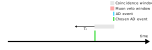
\includegraphics{ap_acc_derivation/timeline_a}
        \caption{Scenario (a)}
    \end{subfigure} \\
    \begin{subfigure}{\textwidth}
        \includegraphics{ap_acc_derivation/timeline_b}
        \caption{Scenario (b)}
    \end{subfigure} \\
    \begin{subfigure}{\textwidth}
        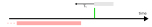
\includegraphics{ap_acc_derivation/timeline_c}
        \caption{Scenario (c)}
    \end{subfigure}
    \caption{The three scenarios used to compute $P_{\text{start}}$}
    \label{fig:ap_scenarios}
\end{figure}
The final formula used for the probability of starting a coincidence window
$P_{\text{start}}$ is the sum of these three terms.

Combining this probability with the other factors gives the following formula
for the probability of an \fold{n} coincidence assuming only
uncorrelated AD events and uncorrelated muons,
neglecting the possibility of correlated pairs or muon-correlated events:

\begin{align} \label{eq:rnfold}
    \begin{split}
        R_{\text{\fold{n}}}
          &= R_s P_{\text{start}} \text{Poisson}(0\vert R_s\tc) \\
          &= R_s \frac{(R_s\tc)^n}{n!} e^{-R_s\tc}
          \left(
              e^{-(R_s + R_\mu)\tc} +
              \frac{R_s}{R_s+R_\mu} e^{-R_\mu\tc}
              \left(
                  1 - e^{-(R_s + R_\mu)\tc}
              \right)
          \right. \\
          &\ \ \left. - \frac{R_s}{2R_s + R_\mu} e^{-R_\mu\tc}
          \left(
              1 - e^{-(2R_s + R_\mu)\tc}
          \right) +
          \frac{R_\mu}{R_s + R_\mu}
          \left(
              1 - e^{-(R_s + R_\mu)\tc}
          \right)
      \right)
    \end{split}
\end{align}

\section{Precision}
\label{ap:singlesprecision}

Values for the three components of $P_{\text{start}}$
under typical near-hall and far-hall scenarios
are given in \cref{tab:pstartcomponents}.
As may be expected given the low singles and muon
rates compared to $\nicefrac{1}{\tc}$,
the most likely situation is that any given AD event
is isolated, corresponding to $P_a$.
The next-most-likely scenario is that the given AD event
is relatively close to a preceding muon veto window,
corresponding to $P_c$.
Since the situation corresponding to $P_b$ requires
not only the given AD event but also 2 others,
all within a time interval shorter than $2\tc$,
it is not surprising that $P_b\ll P_c (< P_a)$
at both the near and far sites.

\begin{figure}
    \includegraphics{ap_acc_derivation/timeline_bad}
    \caption{
        This physical situation is included in $P_b$,
        but it does not lead to our chosen AD event
        starting a coincidence window.
        $P_{\text{start, better}}$ excludes situations like this,
        but it does not make much of a difference
        in the final result for anything measurable
        (see \cref{tab:pstartcomponents}).
    }
    \label{fig:ap_timeline_bad}
\end{figure}

While $P_a$ and $P_c$ are exact mathematical representations
of the corresponding physical scenarios,
$P_b$ is just an approximation stemming from the fact that
the description of the scenario is incomplete.
Recall that $P_b$ is the probability that the given event E0
is preceded by both E1 within \tc{} and E2 further in the past,
configured in such a way that E1 lies inside E2's coincidence window,
and E0 lies outside it.
Missing from this description is that E2 itself must not lie
within a previous event's coincidence window.
(If it did, then E1 would start its own coincidence window
that contains E0, as in \cref{fig:ap_timeline_bad}.)
This could happen for 2 reasons: either (1) there are no events
within \tc{} before E2, (2) there is an event E3 within \tc{}
of E2, and also another event E4 before E3 such that
E3 lies within E4's coincidence window but E2 does not,
or (3) there is a muon but no AD events within \tc{} before E2.
These three scenarios are exactly the same as the original three
describing the possibilities for E0.
It is not too difficult to realize that there is an infinite nesting
of scenarios based around (2), that is, around $P_b$.

In other words, $P_{\text{start}}$ should really be computed as

\begin{align*}
    \begin{split}
        P_{\text{start, better}} &= P_a + P_c + P_b(P_a +
            P_c + P_b(P_a+P_c+P_b(\cdots))) \\
                                 &= P_a + P_c + P_bP_{\text{start, better}},
    \end{split}
\end{align*}
where the second line is obtained by observing that the value
of the infinitely-nested terms in parentheses is simply $P_{\text{start, better}}$.
Solving for $P_{\text{start, better}}$ we obtain the slightly better approximation

\begin{equation}
    P_{\text{start, better}} = \frac{P_a + P_c}{1-P_b}.
\end{equation}

For both the near and far halls, the relative difference
between $P_{\text{start}}$ and $P_{\text{start, better}}$ is $O(10^{-5})$,
so even though $P_{\text{start, better}}$ is still not exact,
further adjustments to it are not necessary.
Why is it not exact?
The description of the physical scenario is once more not complete.
Technically, an AD event \textit{could} occur before E2 in such a way
that E0 would still be able to start a new coincidence window.
This is possible if the hypothetical E3 is very close before E2,
so that E3's coincidence window still contains E1.
The probability of E3 and E2 being ``close enough together''
is strictly less than the probability of E3 occurring anywhere
within \tc{} of E2, which is $\text{Poisson}(1\vert R_s\tc) = 0.028$.
So this correction would be less than a \SI{3}{\percent} correction
to the already negligible $10^{-5}$ correction on $P_{\text{start}}$.

\begin{table}[ht]
    \centering
    \begin{tabular}[t]{lll}
        \hline
        & Near hall & Far hall \\
        \hline
        \tc & \multicolumn{2}{c}{\SI{1500}{\micro\second}} \\
        $R_s$ & \multicolumn{2}{c}{\SI{19}{\hertz}} \\
        $R_\mu$ & \SI{200}{\hertz} & \SI{16}{\hertz} \\
        \hline
        $P_a$ & \num{0.72000} & \num{0.94885} \\
        $P_b$ & \num{0.00024} & \num{0.00038} \\
        $P_c$ & \num{0.25571} & \num{0.02338} \\
        $P_{\text{start}}$ & \num{0.97595} & \num{0.97261} \\
        $P_{\text{start, better}}$ & \num{0.97594} & \num{0.97260} \\
        \hline
    \end{tabular}
    \caption{Values for each component of $P_{\text{start}}$
    for typical $R_\mu$ and $R_s$ at the near and far halls.}
    \label{tab:pstartcomponents}
\end{table}


